\documentclass[25pt, a0paper, landscape]{tikzposter}
\tikzposterlatexaffectionproofoff
\usepackage[utf8]{inputenc}
\usepackage{amsmath}
\usepackage{graphicx}

\title{EHT and black hole fact sheet}
\author{Leo C. Stein}
%\date{\today}
%\institute{ShareLaTeX Institute}

\usepackage{comment}

% \usetheme{Rays}
% \usetheme{Board}
\usetheme{Simple}

\begin{document}

\maketitle

\linespread{1.25}

\begin{columns}
  \column{0.5}
  \block{Units}
    {
      In $G=c=1$ units, masses and lengths and times are all the same.
      \begin{align*}
        \text{Mass of Sun} = M_{\odot} \approx 2\cdot 10^{30} \text{ kg}
        \approx 1.5 \text{ km} \approx 5 \, \mu\text{s}
      \end{align*}
      Astronomical distances are typically measured in AU, parsec, or
      light-year, depending on context
      \begin{align*}
        1 \text{ AU} &\approx 1.5\cdot 10^8 \text{ km} && \text{(Pluto is at $\sim$40 AU)} \\
        1 \text{ pc} &\approx 3 \text{ ly} \approx 3\cdot 10^{13}\text{ km}	&&	\text{(distance to Alpha Cen is 1.3 pc)}
      \end{align*}
      Angles can be measured in radians ($2\pi$ around a circle), or
      arcseconds (1/3600$^{\text{th}}$ of a degree)
      \begin{align*}
        1 \text{ rad} \approx 206\,265 \text{ arcsec}
      \end{align*}

    }
    \block{Black hole basics}
    {\setlength{\parskip}{1cm plus 4mm minus 3mm}

      The Schwarzschild radius is the characteristic size of a black
      hole, and it is \emph{linear} with the BH’s mass (contrast with
      constant density objects).
        \begin{align*}
          R_{s} &= 2\frac{GM}{c^{2}} & \text{(in $G=c=1$ units, simply $R_s = 2M$)}
        \end{align*}
      The event horizon of a non-spinning BH is located at the
      Schwarzschild radius (everything below will be for a
      non-spinning BH). Nothing can return from the event horizon, not
      even light.

      Objects can orbit a BH without being sucked in as long as they
      are not too close. The innermost stable circular orbit (ISCO)
      for matter is at
      \begin{align*}
        R_{\text{ISCO}} = 6M
      \end{align*}
      Because black holes are the curvature of spacetime’s geometry,
      light gets ``deflected'' as it moves around the BH. The most
      light-deflection possible is if light goes in an orbit. Light
      can only have unstable orbits, at the ``photon sphere'' or
      ``light ring''
      \begin{align*}
        R_{\text{ph}} = 3M
      \end{align*}

      This orbit is unstable: A light ray that orbits just outside
      $R_{\text{ph}}$ will spiral out to infinity where we can see it. But
      because of light deflection, it \emph{looks} like it came from a larger
      radius, the critical impact parameter or ``capture radius''
      \begin{align*}
        R_{c} =\sqrt{27}M \approx 5M
      \end{align*}

      Black holes themselves don’t emit any light. They must be
      detected by their influence on nearby matter and light, most
      commonly infalling matter in an ``accretion disk.'' Matter
      slowly spirals inward (because of hydrodynamics, not because the
      BH is ``sucking'') until it gets to about $R_{\text{ISCO}}$, and
      then plunges toward and through the event horizon. This
      matter gets hotter and brighter as it gets closer in; most of
      the emission comes from near $R_{\text{ISCO}}$.
      % The time for matter to orbit at $R_{\text{ISCO}}$ sets a
      % characteristic time for imaging.

      Even though most of the light is emitted near $R_{\text{ISCO}}$,
      light rays can skim the photon orbit and come back out; they
      seem to originate from $R_{\text{ph}}$, meaning they \emph{appear} as a
      ring with radius $R_{c}$. This is the \textbf{black hole
        shadow}. Almost no light comes from inside $R_c$.
    }

    \column{.2}
    \block{}{

      \vspace{8em}

      The shadow of M87 A*. \\
      Credit: Event Horizon Telescope Collaboration
      \vspace{.3em}
      \begin{center}
        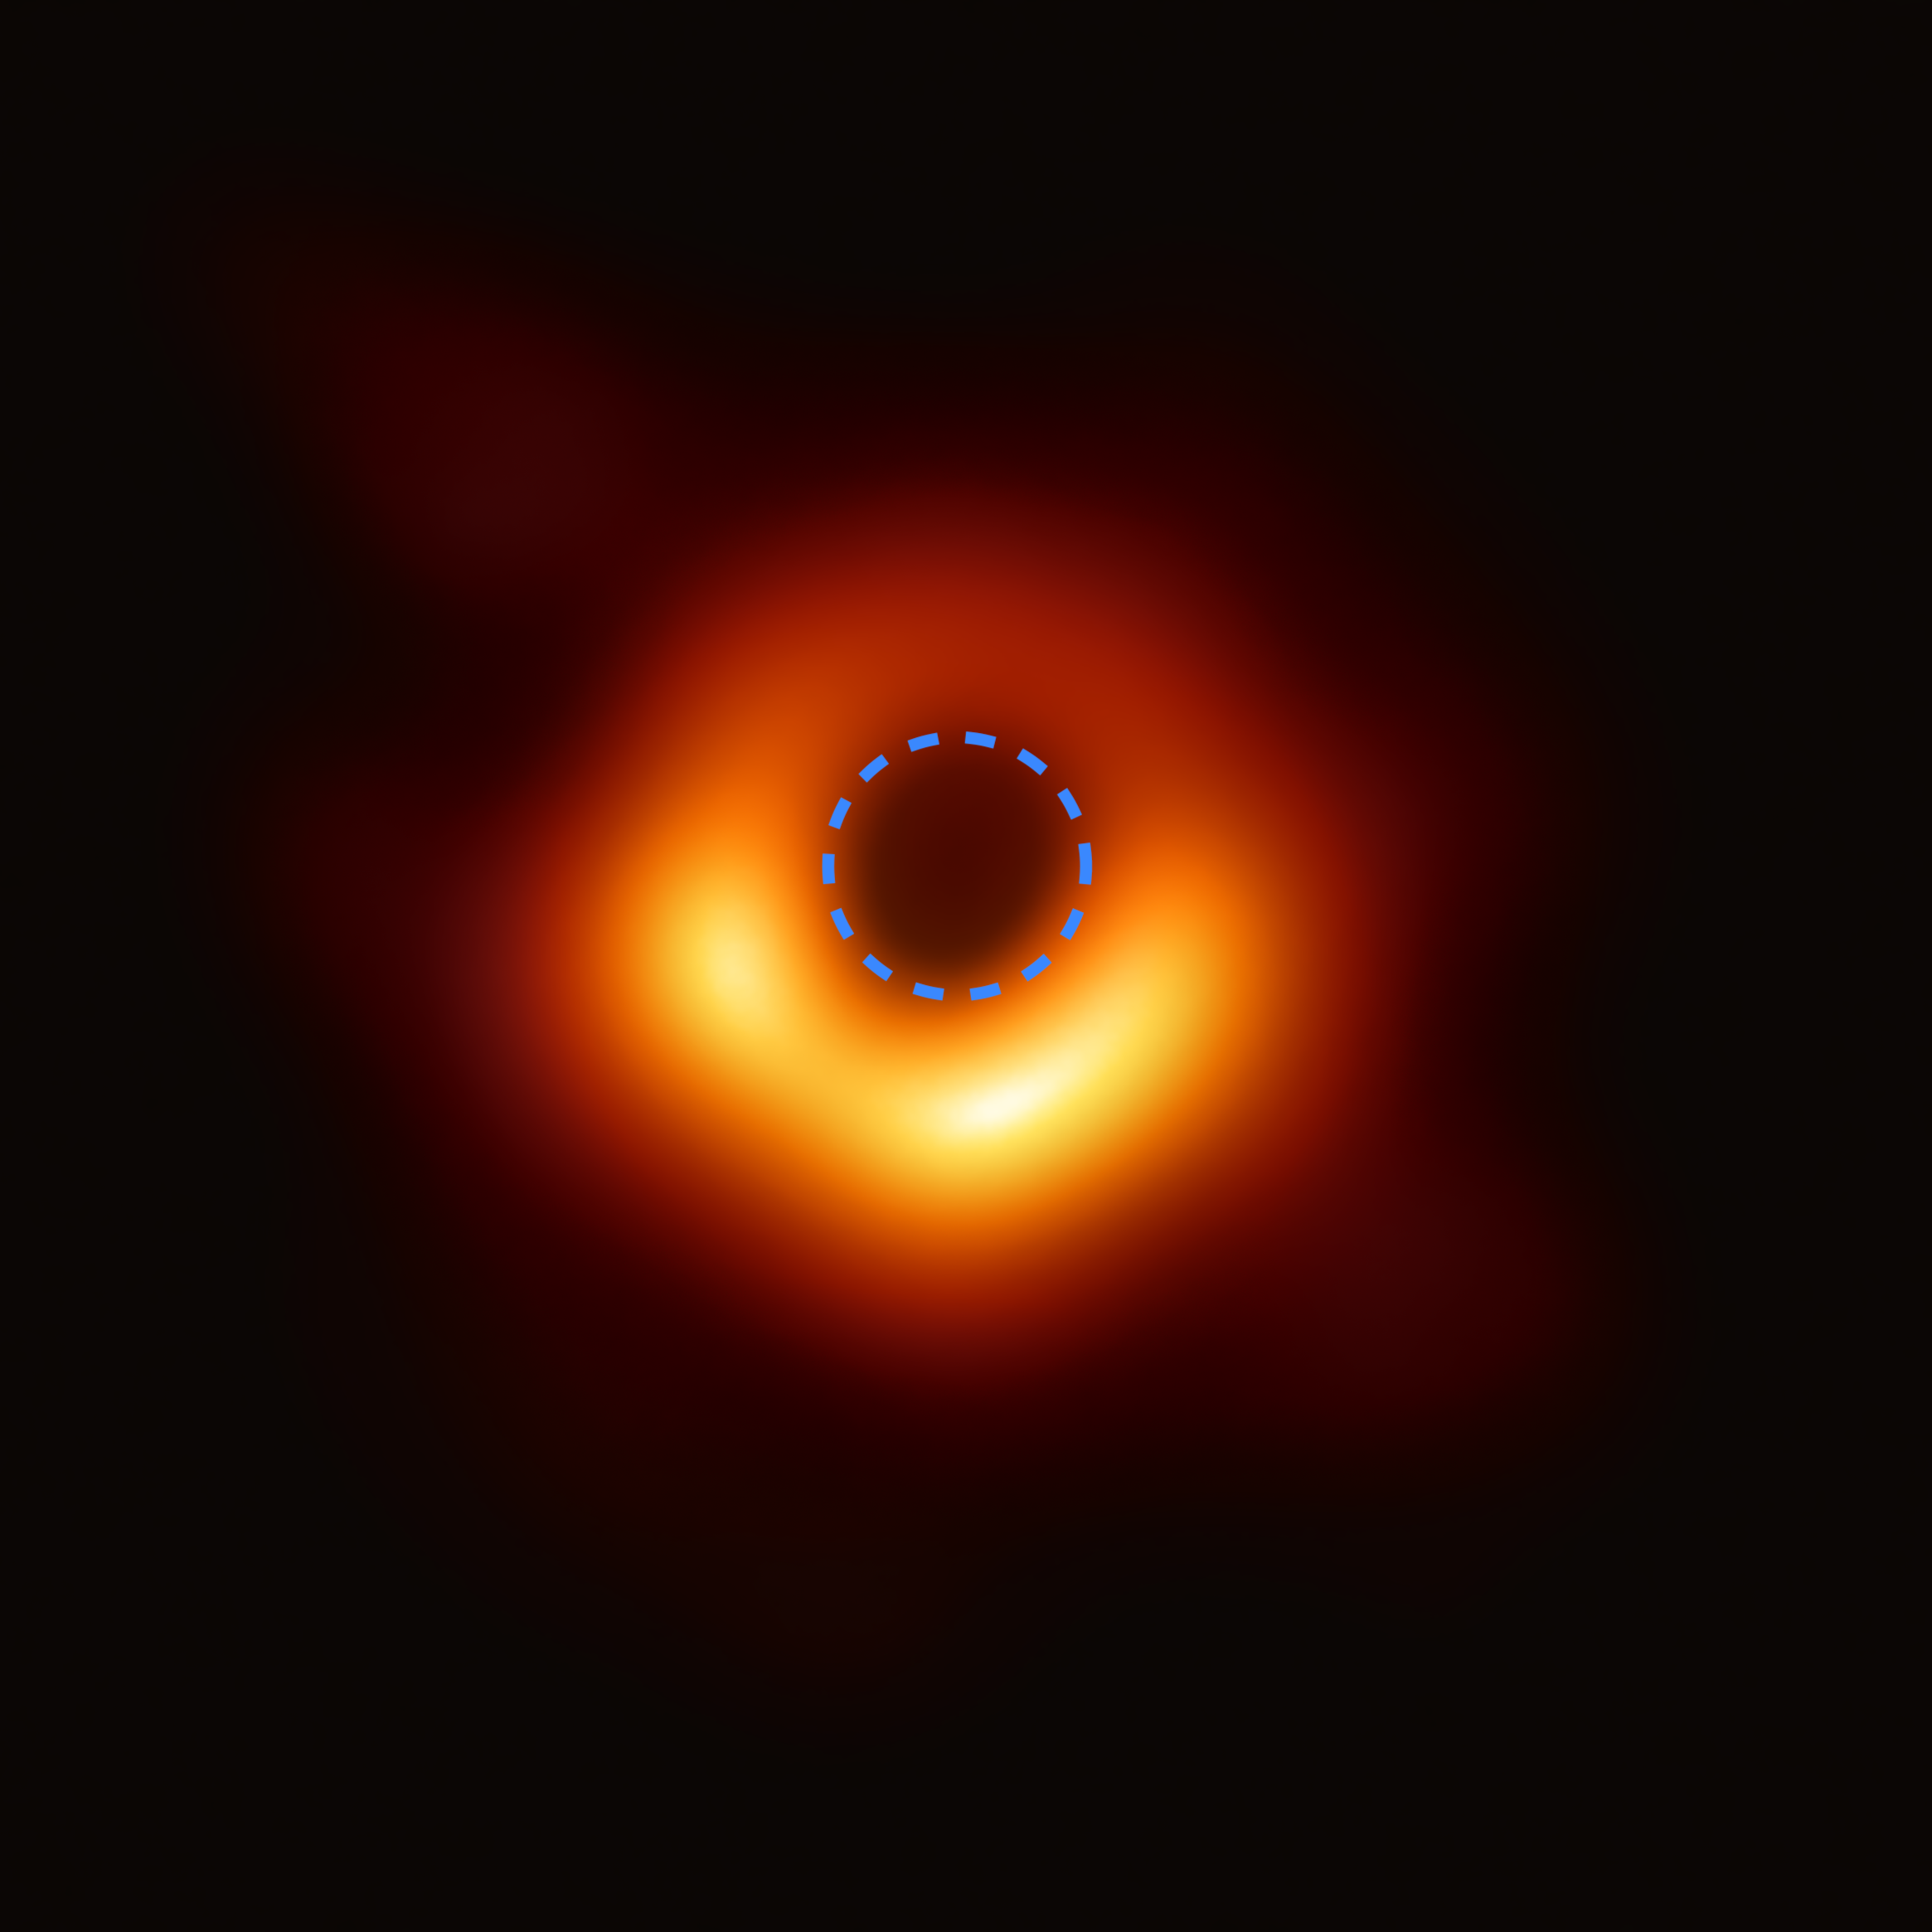
\includegraphics[width=20em, trim={10cm 10cm 10cm 10cm}, clip]{m87a-img-square}

        \vspace{1em}

        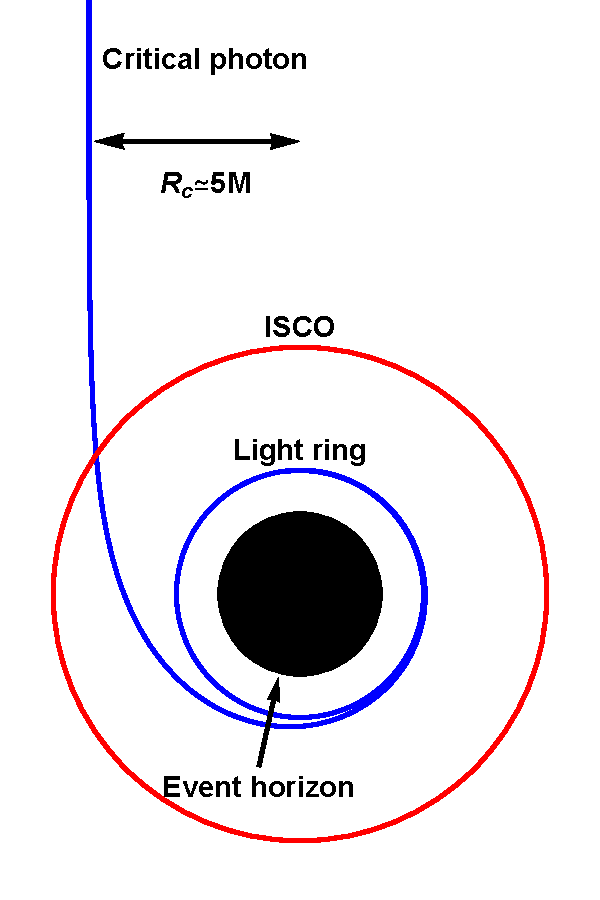
\includegraphics[width=20em]{bh-dist-fig}
      \end{center}

    }

    \column{0.3}
    \block{Imaging}
    {
      Suppose you try to image a BH with a telescope of diameter
      $D_{\text{tel}}$, using light of wavelength $\lambda$. The
      telescope resolution is given by \emph{Rayleigh’s criterion},
      \begin{align*}
        \theta_{\text{res}} \approx \frac{\lambda}{D_{\text{tel}}}
      \end{align*}
      If a BH is at a very large distance $D_{\text{BH}}$, and the
      shadow has diameter $d_{s}=2R_{c}\approx 10GM/c^{2}$, the shadow
      will subtend an angle
      \begin{align*}
        \theta_{s} \approx \frac{d_{s}}{D_{\text{BH}}} \approx \frac{10 M}{D_{\text{BH}}}
      \end{align*}
      If you want to be able to tell there is a shadow, you need the
      telescope’s angular resolution $\theta_{\text{res}}$ to be (at
      least) a few times smaller than the BH’s shadow angle
      $\theta_{s}$.

      If you use $\lambda=1.3$ mm radio waves, and make the whole Earth
      your telescope, $D_{\text{tel}} \approx 1.3\cdot 10^{4}$ km,
      your limit will be
      \begin{align*}
        \theta_{\text{res}} \approx 10^{-10} \text{ rad} \approx 20 \,\mu\text{arcsec}
      \end{align*}

    }

    \block{EHT targets}
    {
      \innerblock{Sgr A*}{
        Sgr A* is the name of the supermassive black hole (SMBH) in
        our own Milky Way galaxy. It has a mass of
        \begin{align*}
          M_{\text{Sgr A*}} \approx 4\cdot10^6 M_\odot \approx 6\cdot10^6\text{ km} \approx 20\text{ s}
        \end{align*}
        The separation between Earth and Sgr A* is
        \begin{align*}
          D_{\text{Sgr A*}} \approx 7.8 \text{ kpc} \approx 2.5\cdot10^{17}\text{ km}
        \end{align*}
        The expected shadow size is
        \begin{align*}
          \theta_{\text{Sgr A*}} \approx \frac{10M_{\text{Sgr A*}}}{D_{\text{Sgr A*}}}
          \approx 2.4\cdot10^{-10}\text{ rad} \approx 50 \, \mu\text{arcsec}
        \end{align*}
        This is a bit bigger than $\theta_{\text{res}}$ for the Earth
        at 1.3 mm wavelength.
      }
      \vspace{1em}
      \innerblock{M87 A*}{
        M87 A* is the SMBH in the galaxy M87, which is in the Virgo
        cluster. It is roughly a thousand times more massive and thus
        bigger than Sgr A*. However it is also roughly a thousand
        times farther away, so it is about the same angle on the
        sky.
        \begin{align*}
          M_{\text{M87 A*}} &\approx 6.5\cdot10^9 M_\odot \approx 10^{10}\text{ km}
          \approx 66\text{ AU} \approx 9\text{ hr} \\
          D_{\text{M87 A*}} &\approx 16.8\text{ Mpc} \approx
          5\cdot10^{20}\text{ km} \approx 55 \text{ million lyr}\\
          \theta_{\text{M87 A*}} &\approx
          \frac{10 M_{\text{M87 A*}}}{D_{\text{M87 A*}}}
          \approx 2.4\cdot10^{-10} \text{rad} \approx 40 \, \mu\text{arcsec}
        \end{align*}
        This is barely bigger than $\theta_{\text{res}}$ for the
        Earth at 1.3 mm wavelength.
      }
    }
\end{columns}

\end{document}
